% !TeX spellcheck = ru_RU
% !TEX root = vkr.tex

\section{Обзор}
\label{sec:relatedworks}

Настоящая работа продолжает исследование, начатое в бакалаврской работе Абросимова~\cite{abrosimov2025cinderella}, в которой были реализованы алгоритмы CINDERELLA и PLI-CIND и выполнена их первоначальная интеграция в Desbordante. Для того чтобы данный текст был самодостаточным, ниже приводятся необходимые определения и описания алгоритмов.

\subsection{Условные зависимости включения}

\subsubsection{Основные обозначения}

Пусть $R_1, R_2$~--- реляционные схемы над фиксированными наборами атрибутов $A_1, A_2, \ldots, A_k$. Множество допустимых значений каждого атрибута $A$ обозначим как $\operatorname{dom}(A)$. Пусть $I_1, I_2$~--- экземпляры схем $R_1, R_2$ соответственно. Каждый экземпляр $I$ состоит из набора кортежей $t$ таких, что $t[A] \in \operatorname{dom}(A)$ для каждого атрибута $A \in R$. Пусть $X, X_P$~--- множества атрибутов $R_1$, а $Y, Y_P$~--- множества атрибутов $R_2$. Обозначим за $t[X]$ проекцию кортежа $t$ на атрибуты $X$.

\emph{Замечание.} На практике $I_1, I_2$ представляют собой таблицы в реляционной базе данных, а $t$~--- строку таблицы.

\subsubsection{Зависимость включения}

\textbf{Определение 1} (Зависимость включения). \emph{Зависимостью включения (Inclusion Dependency, IND) называется отношение $R_1[X] \subseteq R_2[Y]$, которое выполняется на всей таблице. То есть, $\forall\, t_1 \in I_1 \;\; \exists\, t_2 \in I_2 : t_1[X] = t_2[Y]$.}

Содержательно IND означает, что множество значений атрибутов $X$ в первой таблице является подмножеством значений атрибутов $Y$ во второй. Кортеж $t_1 \in I_1$ \emph{удовлетворяет} IND, если существует ссылочный кортеж $t_2 \in I_2$, для которого $t_1[X] = t_2[Y]$. Атрибуты $X$ и $Y$ называются \emph{атрибутами включения}.

На рис.~\ref{fig:ind_example} представлен пример зависимости включения. Каждое значение столбца $\mathit{PK}$ таблицы $\mathit{Table1}$ присутствует в столбце $\mathit{PK}$ таблицы $\mathit{Table2}$, что формально записывается как IND $\mathit{Table1}[\mathit{PK}] \subseteq \mathit{Table2}[\mathit{PK}]$. Стрелки на рисунке показывают, какому кортежу из $\mathit{Table2}$ соответствует каждый кортеж из $\mathit{Table1}$.

\begin{figure}[h]
\centering
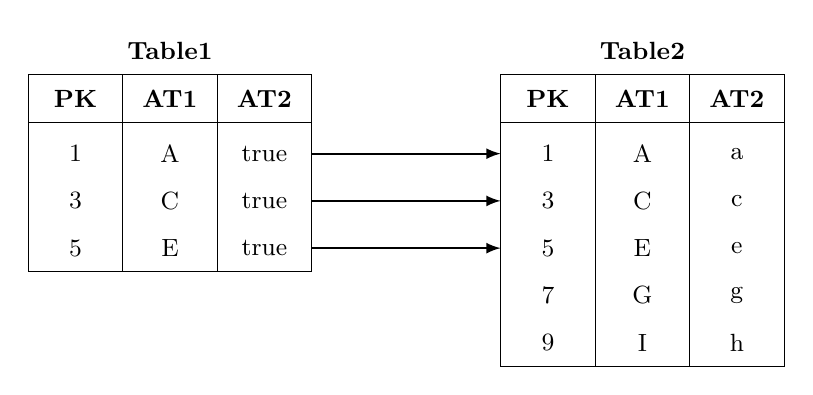
\begin{tikzpicture}[
    every node/.style={font=\small},
    header/.style={font=\small\bfseries, minimum height=6mm},
    cell/.style={minimum width=12mm, minimum height=6mm, anchor=center},
    arr/.style={->, >=latex, thick} 
]
% Table1
\node[header] at (0, 0) {Table1};
\node[header] at (-1.2, -0.6) {PK};
\node[header] at (0, -0.6) {AT1};
\node[header] at (1.2, -0.6) {AT2};
\draw (-1.8, -0.9) -- (1.8, -0.9);
\draw (-1.8, -0.3) -- (1.8, -0.3);
\node[cell] (t1r1) at (-1.2, -1.3) {1};
\node[cell] at (0, -1.3) {A};
\node[cell] at (1.2, -1.3) {true};
\node[cell] (t1r2) at (-1.2, -1.9) {3};
\node[cell] at (0, -1.9) {C};
\node[cell] at (1.2, -1.9) {true};
\node[cell] (t1r3) at (-1.2, -2.5) {5};
\node[cell] at (0, -2.5) {E};
\node[cell] at (1.2, -2.5) {true};
\draw (-1.8, -0.3) rectangle (1.8, -2.8);
\draw (-0.6, -0.3) -- (-0.6, -2.8);
\draw (0.6, -0.3) -- (0.6, -2.8);

% Table2
\node[header] at (6, 0) {Table2};
\node[header] at (4.8, -0.6) {PK};
\node[header] at (6, -0.6) {AT1};
\node[header] at (7.2, -0.6) {AT2};
\draw (4.2, -0.9) -- (7.8, -0.9);
\draw (4.2, -0.3) -- (7.8, -0.3);
\node[cell] (t2r1) at (4.8, -1.3) {1};
\node[cell] at (6, -1.3) {A};
\node[cell] at (7.2, -1.3) {a};
\node[cell] (t2r2) at (4.8, -1.9) {3};
\node[cell] at (6, -1.9) {C};
\node[cell] at (7.2, -1.9) {c};
\node[cell] (t2r3) at (4.8, -2.5) {5};
\node[cell] at (6, -2.5) {E};
\node[cell] at (7.2, -2.5) {e};
\node[cell] at (4.8, -3.1) {7};
\node[cell] at (6, -3.1) {G};
\node[cell] at (7.2, -3.1) {g};
\node[cell] at (4.8, -3.7) {9};
\node[cell] at (6, -3.7) {I};
\node[cell] at (7.2, -3.7) {h};
\draw (4.2, -0.3) rectangle (7.8, -4.0);
\draw (5.4, -0.3) -- (5.4, -4.0);
\draw (6.6, -0.3) -- (6.6, -4.0);

% Arrows
\draw[arr] (1.8, -1.3) -- (4.2, -1.3);
\draw[arr] (1.8, -1.9) -- (4.2, -1.9);
\draw[arr] (1.8, -2.5) -- (4.2, -2.5);
\end{tikzpicture}
\caption{Пример IND: $\mathit{Table1.PK} \subseteq \mathit{Table2.PK}$}
\label{fig:ind_example}
\end{figure}

Зависимости включения играют центральную роль при обнаружении внешних ключей~\cite{rostin2009framework} и поддержании ссылочной целостности~\cite{levene2000justification}. Задача автоматического поиска всех выполняющихся IND является NP-трудной~\cite{kantola1992discovering}.

\subsubsection{Приближённая зависимость включения}

На практике зависимости включения далеко не всегда выполняются на всех данных. Для описания таких случаев вводится ослабленное понятие приближённой зависимости включения.

\textbf{Определение 2} (Приближённая зависимость включения). \emph{Приближённой зависимостью включения (Approximate INclusion Dependency, AIND) называется такая IND, которая выполняется на непустом подмножестве кортежей из $I_1$. То есть, $\exists\, t_1 \in I_1, t_2 \in I_2 : t_1[X] = t_2[Y]$. Обозначается как $R_1[X] \subseteq' R_2[Y]$.}

Приближённая зависимость включения обладает своей метрикой ошибки, которая определяет долю кортежей, на которых зависимость не выполняется.

\textbf{Определение 3} (Ошибка AIND). \emph{Ошибкой AIND называют число $\varepsilon \in [0, 1]$, показывающее долю кортежей, на которых соответствующая IND не выполняется. Вычисляется по формуле:}
\[
\varepsilon = 1 - \frac{|I_1[R_1[X] \subseteq' R_2[Y]]|}{|I_1|},
\]
\emph{где $I_1[R_1[X] \subseteq' R_2[Y]]$~--- множество всех кортежей из $I_1$, для которых зависимость $R_1[X] \subseteq R_2[Y]$ выполняется.}

На рис.~\ref{fig:aind_example} представлен пример приближённой зависимости включения. Кортежи со значениями $\mathit{PK} \in \{1, 3, 5\}$ удовлетворяют IND, а кортежи со значениями $\mathit{PK} \in \{2, 4\}$~--- нет, поскольку значения 2 и 4 отсутствуют в столбце $\mathit{PK}$ таблицы $\mathit{Table2}$. На рисунке невключённые строки выделены цветом. Таким образом, AIND $\mathit{Table1}[\mathit{PK}] \subseteq' \mathit{Table2}[\mathit{PK}]$ выполняется с ошибкой $\varepsilon = 1 - 3/5 = 0{,}4$.

\begin{figure}[h]
\centering
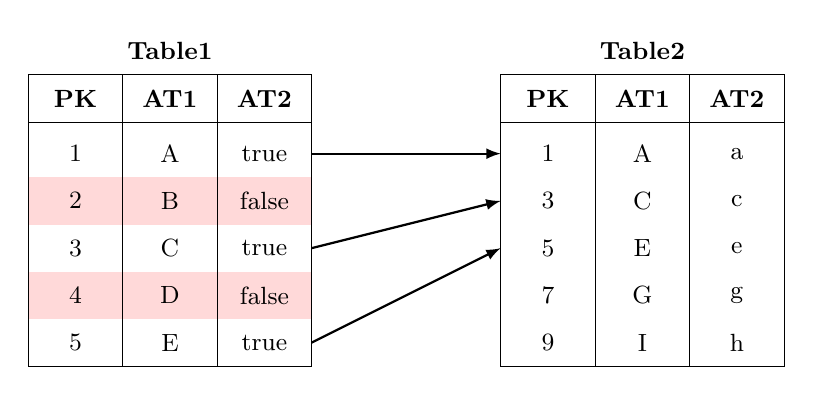
\begin{tikzpicture}[
    every node/.style={font=\small},
    header/.style={font=\small\bfseries, minimum height=6mm},
    cell/.style={minimum width=12mm, minimum height=6mm, anchor=center},
    arr/.style={->, >=latex, thick} 
]
% Table1
\node[header] at (0, 0) {Table1};
\node[header] at (-1.2, -0.6) {PK};
\node[header] at (0, -0.6) {AT1};
\node[header] at (1.2, -0.6) {AT2};
\draw (-1.8, -0.9) -- (1.8, -0.9);
\draw (-1.8, -0.3) -- (1.8, -0.3);
% Row 1 (included)
\node[cell] at (-1.2, -1.3) {1};
\node[cell] at (0, -1.3) {A};
\node[cell] at (1.2, -1.3) {true};
% Row 2 (NOT included) - red background
\fill[red!15] (-1.8, -1.6) rectangle (1.8, -2.2);
\node[cell] at (-1.2, -1.9) {2};
\node[cell] at (0, -1.9) {B};
\node[cell] at (1.2, -1.9) {false};
% Row 3 (included)
\node[cell] at (-1.2, -2.5) {3};
\node[cell] at (0, -2.5) {C};
\node[cell] at (1.2, -2.5) {true};
% Row 4 (NOT included) - red background
\fill[red!15] (-1.8, -2.8) rectangle (1.8, -3.4);
\node[cell] at (-1.2, -3.1) {4};
\node[cell] at (0, -3.1) {D};
\node[cell] at (1.2, -3.1) {false};
% Row 5 (included)
\node[cell] at (-1.2, -3.7) {5};
\node[cell] at (0, -3.7) {E};
\node[cell] at (1.2, -3.7) {true};
\draw (-1.8, -0.3) rectangle (1.8, -4.0);
\draw (-0.6, -0.3) -- (-0.6, -4.0);
\draw (0.6, -0.3) -- (0.6, -4.0);

% Table2
\node[header] at (6, 0) {Table2};
\node[header] at (4.8, -0.6) {PK};
\node[header] at (6, -0.6) {AT1};
\node[header] at (7.2, -0.6) {AT2};
\draw (4.2, -0.9) -- (7.8, -0.9);
\draw (4.2, -0.3) -- (7.8, -0.3);
\node[cell] at (4.8, -1.3) {1};
\node[cell] at (6, -1.3) {A};
\node[cell] at (7.2, -1.3) {a};
\node[cell] at (4.8, -1.9) {3};
\node[cell] at (6, -1.9) {C};
\node[cell] at (7.2, -1.9) {c};
\node[cell] at (4.8, -2.5) {5};
\node[cell] at (6, -2.5) {E};
\node[cell] at (7.2, -2.5) {e};
\node[cell] at (4.8, -3.1) {7};
\node[cell] at (6, -3.1) {G};
\node[cell] at (7.2, -3.1) {g};
\node[cell] at (4.8, -3.7) {9};
\node[cell] at (6, -3.7) {I};
\node[cell] at (7.2, -3.7) {h};
\draw (4.2, -0.3) rectangle (7.8, -4.0);
\draw (5.4, -0.3) -- (5.4, -4.0);
\draw (6.6, -0.3) -- (6.6, -4.0);

% Arrows (only for included rows)
\draw[arr] (1.8, -1.3) -- (4.2, -1.3);
\draw[arr] (1.8, -2.5) -- (4.2, -1.9);
\draw[arr] (1.8, -3.7) -- (4.2, -2.5);
\end{tikzpicture}
\caption{Пример AIND: $\mathit{Table1.PK} \subseteq \mathit{Table2.PK}$ с метрикой ошибки $\varepsilon = 0{,}4$}
\label{fig:aind_example}
\end{figure}

Приближённые зависимости дают агрегированную оценку доли нарушений, однако не раскрывают того, \emph{на каком именно подмножестве} данных зависимость выполняется. Для преодоления этого ограничения вводится понятие условной зависимости включения.

\subsubsection{Таблица условий}

Прежде чем определить условную зависимость включения, необходимо ввести понятие таблицы условий~--- центрального компонента, определяющего подмножество кортежей, на которых зависимость должна выполняться.

\textbf{Определение 4} (Таблица условий). \emph{Таблица условий (Pattern Tableau) $T_P$ состоит из кортежей над атрибутами $X_P$ и $Y_P$. Для каждого такого кортежа $t_P$ выполняется:}
\[
\forall\, A \in X_P \cup Y_P : t_P[A] = a \in \operatorname{dom}(A) \;\lor\; t_P[A] = \text{`---'},
\]
\emph{где `---' является специальным значением, обозначающим отсутствие ограничения на данный атрибут. Такие кортежи называются шаблонами, или условиями.}

Говорят, что кортеж $t_1 \in I_1$ \emph{удовлетворяет} условию $t_P$, если $\forall\, A \in X_P : t_1[A] = t_P[A] \;\lor\; t_P[A] = \text{`---'}$. Атрибуты $X_P, Y_P$ называются \emph{атрибутами условия}. Важно, что множества $X$ и $X_P$, а также $Y$ и $Y_P$, не пересекаются.

В качестве примера рассмотрим шаблон $t_P = (\mathit{AT1} = \text{`---'}, \mathit{AT2} = \text{true})$ при $X_P = \{\mathit{AT1}, \mathit{AT2}\}$. Этот шаблон означает: <<атрибут $\mathit{AT1}$ может принимать любое значение, а $\mathit{AT2}$ должен быть равен true>>. Для данных из рис.~\ref{fig:aind_example} условию удовлетворяют кортежи с $\mathit{PK} \in \{1, 3, 5\}$, и все они являются включёнными.

\subsubsection{Условная зависимость включения}

\textbf{Определение 5} (Условная зависимость включения). \emph{Условной зависимостью включения (Conditional INclusion Dependency, CIND) называется отношение вида:}
\[
\varphi : (R_1[X; X_P] \subseteq R_2[Y; Y_P],\; T_P).
\]
\emph{Оно состоит из IND $R_1[X] \subseteq R_2[Y]$, называемой встроенной IND, и таблицы условий $T_P$, которая определяет подмножество кортежей, на которых эта IND должна выполняться.}

CIND $\varphi$ выполняется для экземпляров $I_1, I_2$, если выполнены следующие условия:

\textbf{Условие выбора для $I_1$.} Пусть $t_1 \in I_1$ удовлетворяет какому-либо условию $t_P \in T_P$. Тогда $t_1$ должна удовлетворять встроенной IND.

\textbf{Условие требования для $I_2$.} Пусть $t_1 \in I_1$ удовлетворяет условию $t_P \in T_P$ и встроенной IND, то есть $\exists\, t_2 \in I_2 : t_1[X] = t_2[Y]$. Тогда $t_2$ также должна удовлетворять $t_P$.

Заметим, что условие выбора для $I_1$ включает в себя условие требования для $I_2$. Более того, шаблон $t_P$, для которого $\forall\, A \in Y_P : t_P[A] = \text{`---'}$, является полностью валидным, то есть условие требования для $I_2$ выполняется тривиально. Поэтому в дальнейшем при поиске CIND будем учитывать только условие выбора для $I_1$.

На рис.~\ref{fig:cind_example} представлен пример CIND. Рассмотрим встроенную IND $\mathit{Table1}[\mathit{PK}] \subseteq \mathit{Table2}[\mathit{PK}]$ и таблицу условий $T_P = \{(\mathit{AT1} = \text{`---'}, \mathit{AT2} = \text{true})\}$. Условию $\mathit{AT2} = \text{true}$ удовлетворяют кортежи с $\mathit{PK} \in \{1, 3, 5\}$. Для каждого из них в $\mathit{Table2}$ существует кортеж с совпадающим значением $\mathit{PK}$, следовательно, условие выбора выполняется и данная CIND валидна. При этом невключённые кортежи ($\mathit{PK} \in \{2, 4\}$) не удовлетворяют условию $\mathit{AT2} = \text{true}$ и потому не нарушают CIND. На рисунке строки, удовлетворяющие условию, выделены цветом.

\begin{figure}[h]
\centering
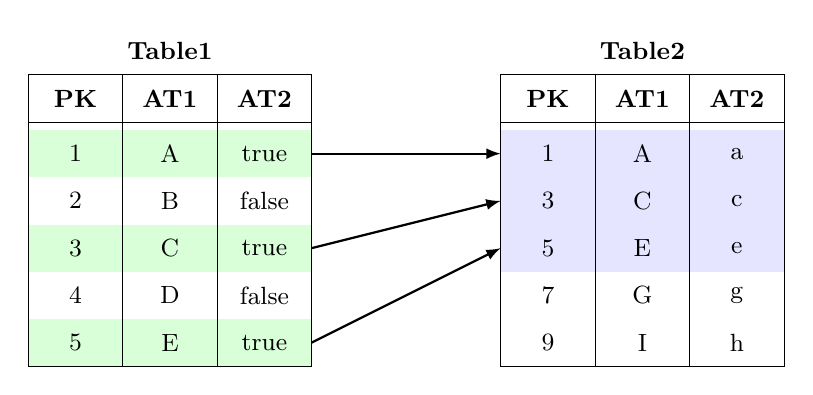
\begin{tikzpicture}[
    every node/.style={font=\small},
    header/.style={font=\small\bfseries, minimum height=6mm},
    cell/.style={minimum width=12mm, minimum height=6mm, anchor=center},
    arr/.style={->, >=latex, thick}  
]
% Table1
\node[header] at (0, 0) {Table1};
\node[header] at (-1.2, -0.6) {PK};
\node[header] at (0, -0.6) {AT1};
\node[header] at (1.2, -0.6) {AT2};
\draw (-1.8, -0.9) -- (1.8, -0.9);
\draw (-1.8, -0.3) -- (1.8, -0.3);
% Row 1 (included, satisfies condition) - green background
\fill[green!15] (-1.8, -1.0) rectangle (1.8, -1.6);
\node[cell] at (-1.2, -1.3) {1};
\node[cell] at (0, -1.3) {A};
\node[cell] at (1.2, -1.3) {true};
% Row 2 (NOT included, does not satisfy condition)
\node[cell] at (-1.2, -1.9) {2};
\node[cell] at (0, -1.9) {B};
\node[cell] at (1.2, -1.9) {false};
% Row 3 (included, satisfies condition) - green background
\fill[green!15] (-1.8, -2.2) rectangle (1.8, -2.8);
\node[cell] at (-1.2, -2.5) {3};
\node[cell] at (0, -2.5) {C};
\node[cell] at (1.2, -2.5) {true};
% Row 4 (NOT included, does not satisfy condition)
\node[cell] at (-1.2, -3.1) {4};
\node[cell] at (0, -3.1) {D};
\node[cell] at (1.2, -3.1) {false};
% Row 5 (included, satisfies condition) - green background
\fill[green!15] (-1.8, -3.4) rectangle (1.8, -4.0);
\node[cell] at (-1.2, -3.7) {5};
\node[cell] at (0, -3.7) {E};
\node[cell] at (1.2, -3.7) {true};
\draw (-1.8, -0.3) rectangle (1.8, -4.0);
\draw (-0.6, -0.3) -- (-0.6, -4.0);
\draw (0.6, -0.3) -- (0.6, -4.0);

% Table2
\node[header] at (6, 0) {Table2};
\node[header] at (4.8, -0.6) {PK};
\node[header] at (6, -0.6) {AT1};
\node[header] at (7.2, -0.6) {AT2};
\draw (4.2, -0.9) -- (7.8, -0.9);
\draw (4.2, -0.3) -- (7.8, -0.3);
% Referenced rows - blue background
\fill[blue!10] (4.2, -1.0) rectangle (7.8, -1.6);
\node[cell] at (4.8, -1.3) {1};
\node[cell] at (6, -1.3) {A};
\node[cell] at (7.2, -1.3) {a};
\fill[blue!10] (4.2, -1.6) rectangle (7.8, -2.2);
\node[cell] at (4.8, -1.9) {3};
\node[cell] at (6, -1.9) {C};
\node[cell] at (7.2, -1.9) {c};
\fill[blue!10] (4.2, -2.2) rectangle (7.8, -2.8);
\node[cell] at (4.8, -2.5) {5};
\node[cell] at (6, -2.5) {E};
\node[cell] at (7.2, -2.5) {e};
\node[cell] at (4.8, -3.1) {7};
\node[cell] at (6, -3.1) {G};
\node[cell] at (7.2, -3.1) {g};
\node[cell] at (4.8, -3.7) {9};
\node[cell] at (6, -3.7) {I};
\node[cell] at (7.2, -3.7) {h};
\draw (4.2, -0.3) rectangle (7.8, -4.0);
\draw (5.4, -0.3) -- (5.4, -4.0);
\draw (6.6, -0.3) -- (6.6, -4.0);

% Arrows (only for rows satisfying the condition)
\draw[arr] (1.8, -1.3) -- (4.2, -1.3);
\draw[arr] (1.8, -2.5) -- (4.2, -1.9);
\draw[arr] (1.8, -3.7) -- (4.2, -2.5);
\end{tikzpicture}
\caption{Пример CIND: $\mathit{Table1.PK} \subseteq \mathit{Table2.PK}$ с таблицей условий $T_P = \{(\mathit{AT1} = \text{`---'},\; \mathit{AT2} = \text{true})\}$}
\label{fig:cind_example}
\end{figure}

\subsubsection{Метрики качества условий}

На практике полностью валидные или полностью полные условия встречаются редко. Для количественной оценки качества условий вводятся две метрики: валидность и полнота. Прежде чем их определить, введём необходимые обозначения.

Пусть дана CIND~$\varphi$ и экземпляры $I_1, I_2$. Обозначим за $I_\varphi$ множество кортежей из $I_1$, удовлетворяющих встроенной IND. Для ненормализованных таблиц существенную роль играют \emph{группы включённых кортежей}. Пусть $g_x = \{t \mid t \in I_1 \wedge t[X] = x\}$~--- группа кортежей из $I_1$, у которых значение на атрибутах включения $X$ равно $x$. Группа называется \emph{включённой}, если хотя бы один кортеж из неё удовлетворяет IND. Обозначим $G_1$~--- множество всех групп в $I_1$, $G_\varphi$~--- множество включённых групп. Наконец, $I[t_P]$~--- множество кортежей из $I$, удовлетворяющих условию $t_P$, а $G[t_P]$~--- множество таких групп.

\textbf{Определение 6} (Валидное условие). \emph{Условие называется валидным, если все кортежи (группы), которые ему удовлетворяют, являются включёнными. Является аналогом точности (precision) классификатора из теории машинного обучения.}

\textbf{Определение 7} (Полное условие). \emph{Условие называется полным, если ему удовлетворяют все включённые кортежи (группы). Для групп такое свойство может также называться покрытием (covering). Является аналогом полноты (recall) классификатора.}

В реальности получить полностью валидные или полные условия практически невозможно. Поэтому определим метрики валидности и полноты как метрики, которые возможно посчитать.

\textbf{Определение 8} (Валидность условия). \emph{Валидность условия $\operatorname{valid}(t_P) \in [0, 1]$ вычисляется по формуле}
\[
\operatorname{valid}(t_P) = \frac{|I_\varphi[t_P]|}{|I_1[t_P]|}
\]
\emph{для строковых условий, и по формуле}
\[
\operatorname{valid}_g(t_P) = \frac{|G_\varphi[t_P]|}{|G_1[t_P]|}
\]
\emph{для групповых. Условие $t_P$ называется $\gamma$-валидным, если его валидность больше $\gamma$.}

\textbf{Определение 9} (Полнота условия). \emph{Полнота условия $\operatorname{completeness}(t_P) \in [0, 1]$ вычисляется по формуле}
\[
\operatorname{completeness}(t_P) = \frac{|I_\varphi[t_P]|}{|I_\varphi|}
\]
\emph{для строковых условий, и по формуле}
\[
\operatorname{completeness}_g(t_P) = \frac{|G_\varphi[t_P]|}{|G_\varphi|}
\]
\emph{для групповых. Условие $t_P$ называется $\delta$-полным, если его полнота больше $\delta$.}

Проиллюстрируем метрики на примере. Вернёмся к данным из рис.~\ref{fig:aind_example}. Условие $t_P = (\mathit{AT2} = \text{true})$ удовлетворяется тремя кортежами из $I_1$: $\{1, 3, 5\}$. Все три являются включёнными, поэтому $\operatorname{valid}(t_P) = 3/3 = 1{,}0$. Включённых кортежей всего три, и все они удовлетворяют условию, поэтому $\operatorname{completeness}(t_P) = 3/3 = 1{,}0$. Данное условие является одновременно полностью валидным и полностью полным.

Теперь рассмотрим условие $t_P' = (\mathit{AT1} = \text{`A'})$. Ему удовлетворяет один кортеж с $\mathit{PK} = 1$, который является включённым: $\operatorname{valid}(t_P') = 1/1 = 1{,}0$. Однако $\operatorname{completeness}(t_P') = 1/3 \approx 0{,}33$~--- условие покрывает лишь треть включённых кортежей.

Используя эти метрики, можно задавать ограничения на найденные условия и фильтровать как те, которые охватывают слишком много невалидных кортежей, так и те, которые применяются на чрезмерно малой выборке данных.

\emph{Замечание: в дальнейшем условия, метрики которых посчитаны для групп, будут называться \textbf{групповыми} условиями. В свою очередь те условия, метрики которых посчитаны для обычного представления таблицы, будут называться \textbf{строковыми} условиями.}

Таким образом, CIND представляет собой составной примитив, состоящий из AIND и таблицы условий. При поиске CIND необходимо сначала обнаружить AIND, а затем для каждой из них отдельно искать подходящие условия. Поскольку алгоритмы поиска AIND уже реализованы в Desbordante, основная задача состоит в оптимизации алгоритмов поиска условий. При этом условия характеризуются валидностью и полнотой, и поскольку полностью валидных и полных условий на практике может не существовать, алгоритмы должны поддерживать пороговые значения $\gamma$ и $\delta$ в качестве параметров. Кроме того, метрики могут вычисляться как для отдельных кортежей (строковые условия), так и для групп кортежей с одинаковыми значениями атрибутов включения (групповые условия), что также должно быть отражено в параметрах алгоритма.

\subsection{Алгоритмы поиска AIND}

Как было отмечено выше, поиск CIND начинается с обнаружения приближённых зависимостей включения. Нахождение всего множества зависимостей включения для заданного набора данных~--- одна из наиболее вычислительно сложных задач профилирования данных~\cite{dursch2019inclusion}. Для её решения разработан ряд специализированных алгоритмов, среди которых наиболее известны следующие:

\begin{itemize}
    \item \textbf{SPIDER}~\cite{bauckmann2006efficiently}~--- алгоритм, основанный на сортировке значений атрибутов и последующем слиянии отсортированных списков. Он не требует загрузки всех данных в оперативную память: отсортированные списки могут храниться на диске и считываться последовательно, что делает его применимым к наборам данных, существенно превышающим объём доступной памяти. Алгоритм эффективно обнаруживает как точные, так и приближённые зависимости включения;

    \item \textbf{BINDER}~\cite{papenbrock2015divide}~--- алгоритм, использующий стратегию <<разделяй и властвуй>> для сокращения пространства поиска. Применяет фильтры Блума для предварительного отсечения заведомо невыполняющихся кандидатов, что позволяет эффективно работать с большими наборами данных;

    \item \textbf{MIND}~\cite{de2002unary}~--- алгоритм поиска унарных зависимостей включения, основанный на инвертированных индексах. Отличается простотой реализации, однако при большом количестве уникальных значений размер индексов существенно возрастает;

    \item \textbf{FAIDA}~\cite{kruse2018fast}~--- алгоритм, использующий хэш-функции для приближённого сравнения множеств значений атрибутов. FAIDA гарантированно находит все выполняющиеся IND, но может выдавать ложноположительные результаты. Ориентирован на поиск точных IND и не поддерживает приближённые зависимости.
\end{itemize}

В Desbordante на момент начала данной работы реализованы SPIDER, FAIDA и MIND. Поскольку для пайплайна CIND необходим алгоритм, способный обнаруживать приближённые зависимости включения, FAIDA не подходит~--- он поддерживает только точные IND. Алгоритм MIND, хотя и позволяет искать AIND, был реализован в Desbordante сравнительно недавно, и его эффективность в рамках данной реализации не была экспериментально подтверждена. По этим причинам в качестве алгоритма поиска AIND для пайплайна CIND был выбран SPIDER~--- он хорошо зарекомендовал себя как для точных, так и для приближённых зависимостей включения, обладает предсказуемым потреблением памяти и уже имеет проверенную реализацию в Desbordante.

\subsection{Алгоритмы поиска условий CIND}

Алгоритмы поиска условий для CIND были впервые представлены в статье Баукманн и др.~\cite{brink2012cind}. Авторы предложили два алгоритма~--- CINDERELLA и PLI-CIND, основанных на различных принципах, но объединённых общей двухфазной архитектурой.

Оба алгоритма принимают на вход результат работы алгоритма поиска AIND~--- список приближённых зависимостей включения. Для каждой найденной AIND алгоритм ищет таблицу условий $T_P$, состоящую из $\gamma$-валидных и $\delta$-полных условий. Ключевое различие между CINDERELLA и PLI-CIND заключается в стратегии поиска кандидатов в условия~--- корректных шаблонов, которые потенциально могут войти в таблицу условий, но метрики качества которых ещё не вычислены.

Оба алгоритма опираются на идею \emph{внешнего левого соединения} (left outer join) двух таблиц по атрибутам включения. Результат такого соединения позволяет для каждого кортежа из $I_1$ определить, является ли он включённым, то есть имеет ли соответствующий кортеж в $I_2$. С целью упрощения дальнейшего изложения каждый алгоритм сначала описывается в версии для поиска групповых условий, а затем указываются модификации для строковых условий.

\subsubsection{Алгоритм CINDERELLA}

Алгоритм Conditional INclusion DEpendency REcognition Leveraging deLimited Apriori (CINDERELLA) основан на поиске ассоциативных правил~\cite{brink2012cind}. Неформально ассоциативные правила имеют такой смысл: <<кто покупает $X$, тот зачастую покупает и $Z$>>. В контексте CINDERELLA эти правила приобретают следующую интерпретацию: <<строки таблицы, чьи значения атрибутов условий равны $x$, как правило, являются включёнными>>.

Для поиска ассоциативных правил используется алгоритм Apriori~\cite{agrawal1994fast}, который представляет таблицу в виде \emph{контейнеров} (baskets). В каждый контейнер помещаются все пары вида $(\text{атрибут условия}, \text{значение})$, соответствующие одной группе (или строке~--- для строковых условий), а также индикатор включения, если соответствующая группа является включённой.

Apriori использует метрики support и confidence для сужения области поиска и вывода нужных правил. В контексте CIND этими метриками выступают полнота и валидность. Область поиска можно сократить по метрике полноты, пользуясь следующим инвариантом: с ростом количества атрибутов в условии его полнота не возрастает. Таким образом, алгоритм получает все наборы кандидатов с необходимой полнотой, после чего фильтрует их по валидности, формируя итоговый список условий.

Алгоритм CINDERELLA основан на одной из вариаций Apriori~--- алгоритме MultipleJoins~\cite{brink2012cind}. Его ключевая оптимизация состоит в том, что нас интересуют только правила, у которых атрибут включения имеет положительное значение, то есть нас интересуют только условия для включённых групп. Благодаря этому CINDERELLA при поиске кандидатов может использовать одно соединение вместо трёх, как в оригинальном MultipleJoins, за счёт чего сильно сужается область поиска кандидатов и повышается производительность.

Опишем работу алгоритма более детально. Пусть $L_k$~--- множество наборов элементов длины $k$, обладающих достаточной полнотой ($\geq \delta$), а $C_k$~--- множество кандидатов в $L_k$.

Для начала за один проход по всем контейнерам вычисляется $L_1$~--- множество отдельных элементов с полнотой не ниже $\delta$. Затем на каждой последующей итерации формируется $C_k$ из $L_{k-1}$: кандидат формируется из двух наборов, у которых первые $k-2$ элементов одинаковы, а последний элемент первого набора меньше последнего элемента второго. Таким образом поддерживается отсортированный порядок элементов в наборе. Далее необходимо определить, является ли получившийся набор элементов корректным: для этого проверяется, что все подмножества длины $k-1$, содержащие индикатор включения, лежат в $L_{k-1}$. У получившихся кандидатов заново вычисляется полнота, и по ней фильтруются наборы, формируя $L_k$. Процесс повторяется до тех пор, пока $L_k$ не окажется пустым.

Получив все наборы элементов с необходимой полнотой, остаётся лишь выбрать из них те, что имеют достаточную валидность. Это можно делать в процессе вычисления полноты каждого набора элементов. Чтобы применять такой алгоритм для поиска строковых условий, достаточно формировать по контейнеру на каждую отдельную строку таблицы, а не на группу.

CINDERELLA осуществляет поиск кандидатов <<в ширину>> (breadth-first), последовательно наращивая длину условий. Это позволяет эффективно отсекать бесперспективные ветви поиска благодаря антимонотонности полноты. Вместе с тем для проверки корректности набора кандидатов на каждом уровне необходимо хранить хеш-таблицы всех предыдущих уровней, что обеспечивает высокую скорость работы ценой значительного потребления оперативной памяти.

\subsubsection{Алгоритм PLI-CIND}

Второй алгоритм~--- PLI-based Algorithm (PLI-CIND)~--- основан на идее пересечения позиционных списков атрибутов (Position Lists Intersection, PLI)~\cite{brink2012cind}. Позиционный список атрибута~--- это преобразованное представление столбца таблицы, в котором каждому значению атрибута $A$ в строке $t$ сопоставляется набор индексов строк (или групп), содержащих это значение. Позиционные списки можно объединять, пересекая их между собой, формируя тем самым позиционные списки для комбинаций значений нескольких атрибутов. Данное представление широко используется в алгоритмах поиска функциональных зависимостей, например TANE~\cite{huhtala1999tane}.

PLI-CIND, в отличие от CINDERELLA, не пытается на каждой итерации искать все условия одинаковой длины. Напротив, он использует поиск <<в глубину>> (depth-first): пытается расширить текущее условие до тех пор, пока это возможно. Алгоритм разбит на две фазы.

\textbf{Фаза 1. Построение позиционных списков.} Первая фаза выполняется за один проход по таблице: для каждого значения каждого атрибута условия строится позиционный список, содержащий только индексы включённых групп (или строк). Каждое значение атрибута проверяется на полноту~--- если бы это значение сформировало условие, имело бы оно достаточную полноту? В итоге остаются только те списки, которые имеют нужную полноту.

\textbf{Фаза 2. Рекурсивный поиск условий.} Рекурсия запускается из каждого атрибута отдельно. Пока текущий позиционный список не пуст, алгоритм пытается расширить его добавлением нового атрибута. Расширение выполняется пересечением текущего списка со списком позиций этого атрибута. В процессе пересчитываются полнота и валидность: полные списки отправляются по рекурсии дальше, а валидные~--- заносятся в ответ.

Реализации для различных типов условий различаются лишь типом индексов, которые используются на первой фазе при формировании позиционных списков: для строковых условий индексами служат номера строк, для групповых~--- номера групп.

\subsubsection{Сравнение алгоритмов}

Объективно лучшего алгоритма среди двух рассмотренных не существует~--- каждый обладает своими преимуществами и ограничениями.

CINDERELLA ищет кандидатов <<в ширину>>, что позволяет существенно снизить область поиска условий. Вместе с тем этот алгоритм должен хранить намного больший объём данных в процессе работы: для проверки правильности набора необходимо хранить кандидатов всех размеров в виде хеш-таблиц, что хоть и позволяет достичь высокой скорости работы, очень сильно повышает потребление памяти.

PLI-CIND, напротив, потребляет память только на поддержание текущего кандидата и его позиционного списка, что делает совокупное потребление памяти не зависящим от числа кандидатов. Однако поиск <<в глубину>> никак не ограничивает область поиска для расширения кандидата, за счёт чего алгоритм не так эффективен по времени.

Таким образом, выбор алгоритма определяется характеристиками конкретной задачи: при ограниченных ресурсах оперативной памяти предпочтительнее PLI-CIND, тогда как при необходимости минимизации времени работы~--- CINDERELLA.

\subsection{Архитектура Desbordante}

Desbordante~\cite{smirnov2025desbordante}~--- высокопроизводительный инструмент профилирования данных с открытым исходным кодом, реализованный на языке C++. Проект разрабатывается группой исследователей из Санкт-Петербургского государственного университета с 2019 года. По своему назначению Desbordante во многом схож с Metanome~\cite{papenbrock2015data}, однако обладает рядом отличительных особенностей: реализация на C++ позволяет использовать низкоуровневые оптимизации, в том числе SIMD-инструкции для векторизации вычислений; инструмент доступен в качестве pip-пакета для языка Python и предоставляет интерфейс командной строки; несмотря на то что проект является более молодым, в нём реализовано большее число примитивов профилирования, чем в Metanome.

Архитектура Desbordante организована в виде многоуровневой системы, общая схема которой представлена на рис.~\ref{fig:desbordante_arch}. На нижнем уровне расположен слой ввода данных, поддерживающий чтение из CSV-файлов и pandas DataFrame. Данные преобразуются в единое внутреннее представление, включающее реляционную схему, систему типов и индексные структуры~--- позиционные списки (PLI) и индексы столбцов. Над слоем данных располагается ядро системы~--- библиотека алгоритмов, организованная вокруг базового класса \texttt{Algorithm}, предоставляющего единый жизненный цикл: загрузка данных, конфигурация параметров, выполнение и получение результатов. Каждый алгоритм реализует поиск или верификацию определённого типа зависимостей. На верхнем уровне находятся пользовательские интерфейсы: Python-биндинги на основе pybind11 и интерфейс командной строки.

\begin{figure}[h]
\centering
\begin{tikzpicture}[
    every node/.style={font=\small},
    layer/.style={draw, rounded corners=3pt, minimum height=10mm, text centered, fill=white},
    arr/.style={->, >=latex, thick}
]
% User interfaces
\node[layer, minimum width=35mm, fill=blue!8] (python) at (-2.2, 5.5) {Python API};
\node[layer, minimum width=35mm, fill=blue!8] (cli) at (2.2, 5.5) {CLI};

% Bindings
\node[layer, minimum width=75mm, fill=gray!8] (bindings) at (0, 4.2) {Python-биндинги (pybind11)};

% Algorithm factory
\node[layer, minimum width=75mm, fill=gray!8] (factory) at (0, 2.9) {Фабрика алгоритмов / Конфигурация};

% Algorithms - main block
\node[layer, minimum width=75mm, minimum height=18mm, fill=green!6] (algoblock) at (0, 1.2) {};
\node[font=\small\bfseries] at (0, 1.85) {Алгоритмы};
\node[font=\footnotesize] at (0, 1.15) {FD \quad IND \quad UCC \quad OD \quad MD \quad AR};
\node[font=\footnotesize] at (0, 0.55) {CIND \quad DC \quad DD \quad GFD \quad CFD};

% Data model
\node[layer, minimum width=75mm, fill=yellow!8] (model) at (0, -0.5) {Модель данных (схема, типы, PLI)};

% Data input
\node[layer, minimum width=35mm, fill=orange!8] (csv) at (-2.2, -1.8) {CSV-парсер};
\node[layer, minimum width=35mm, fill=orange!8] (df) at (2.2, -1.8) {pandas DataFrame};

% Arrows
\draw[arr] (python) -- (bindings);
\draw[arr] (cli) -- (bindings);
\draw[arr] (bindings) -- (factory);
\draw[arr] (factory) -- (algoblock);
\draw[arr] (algoblock) -- (model);
\draw[arr] (csv) -- (model);
\draw[arr] (df) -- (model);
\end{tikzpicture}
\caption{Архитектура инструмента Desbordante}
\label{fig:desbordante_arch}
\end{figure}

На момент начала данной работы в Desbordante реализована поддержка более 30 алгоритмов поиска и верификации зависимостей данных, включая функциональные зависимости (FD), зависимости включения (IND), уникальные комбинации столбцов (UCC), порядковые зависимости (OD), зависимости соответствия (MD), ассоциативные правила (AR) и ряд других примитивов. Поддержка условных зависимостей включения (CIND) была добавлена в рамках бакалаврской работы~\cite{abrosimov2025cinderella}, однако реализованные алгоритмы не были оптимизированы по производительности, а задача верификации CIND не рассматривалась. Настоящая работа посвящена оптимизации этих алгоритмов и реализации верификатора CIND.

